In October 2012 DASL received officially become a Track-A team for the DRC.
The team is now called DRC-Hubo.
In December 2012 Hubo-Ach was chosen as the primary controller for the DRC-Hubo team.
This would be another source of verification and validation of the Hubo-Ach system.

One of the keys to the team's success is collaboration.
The DRC-Hubo team consists of Drexel University, WPI, Georgia Tech, University of Delaware, Swarthmore, Purdue, Ohio State (check that) and RAINBOW (a company that rose from the Hubo Lab at Korea Advanced Institute of Science and Technology (KAIST)).
Each partner would be responsible with one event.
Efforts will then combine creating one master controller that is capable of doing all the given tasks.
Having this unified framework gives them the ability to share their controllers without having to integrate their code.  

\begin{figure}[thpb]
  \centering
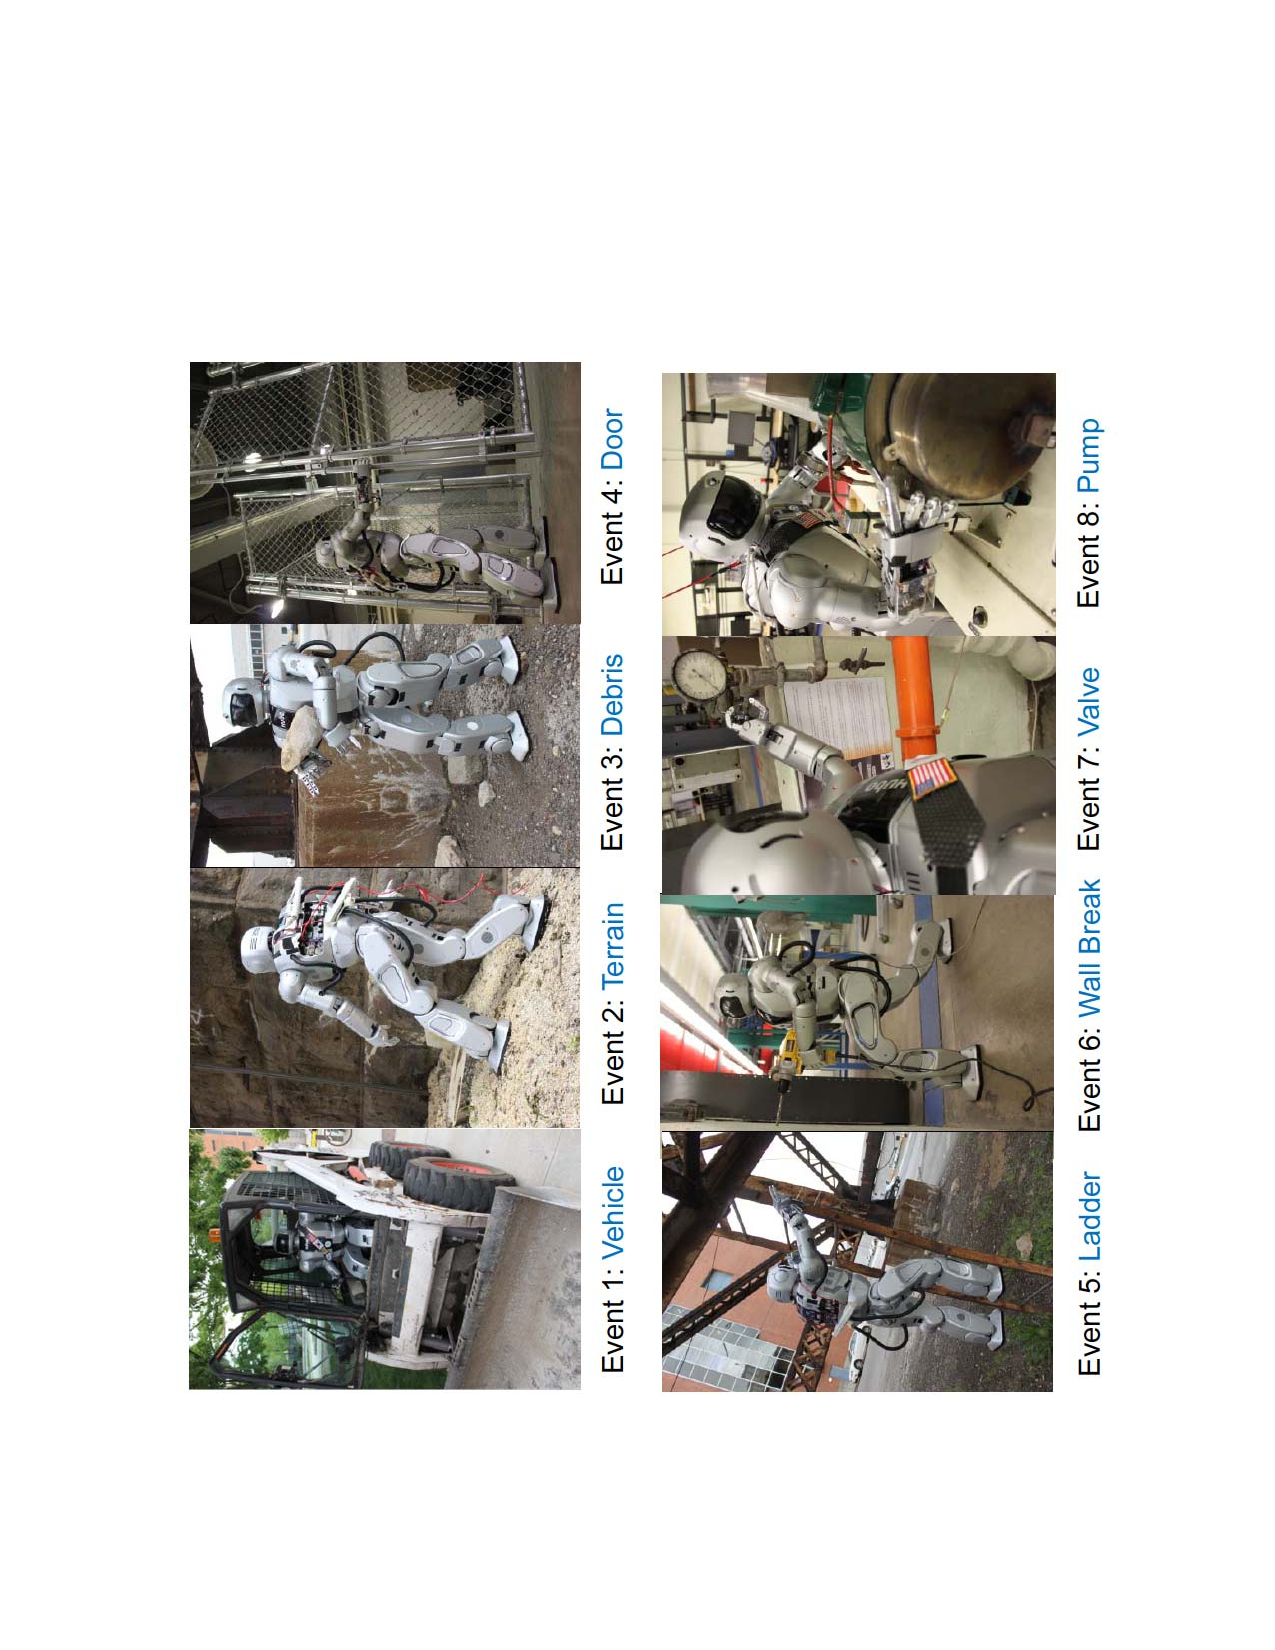
\includegraphics[height=1.0\columnwidth, angle=-90]{./background/pix/drcEvents.pdf}
  \caption{DARPA Robot Challenge Events.  Pictures depict the Hubo2+ (KHR-4) preforming the eight given tasks.  The photographs are meant to help you \textit{imagine} that the robot is capable of preforming these tasks.  The events are - Event 1: Driving an un-modified human vehicle; Event 2: Walking over rough, un-even terrain; Event 3: Removing debris from regions of interest; Event 4: Opening and navigating through multiple doors and hallways; Event 5: Climb an industrial ladder; Event 6: Break through a wall using un-modified human tools; Event 7: Turn a valve; Event 8: Replace a pump (note: this was replaced by a hose insertion task).  All photographs were staged and taken by Daniel M. Lofaro.  Picture montage taken from Dr. Paul Oh's meeting to DARPA at the DRC Kickoff meeting, October 23-25, 2012.\cite{drOhDARPA}    }
  \label{fig:drcEvents}
\end{figure}

